The following chapter is about the SmartAlvarTagDetection component. It is only a brief description of the component and for more details the Technical Report of 2017 \cite{TR17} is recommended. 

\subsubsection{Overview}


The SmartAlvarTagDetection was implemented by the former Robocup team. The component is a crucial component because it identifies the Alvar Tags on the MPS machines. With those Alvar Tags, the robot can identify the machine name and wether the robot is facing the front or back side of the machine. The actual component deals with four types of the MPS machines: Base Station, Cap Station, Ring Station and Storage Station. Therefor a lookup table in the component holds 14 machines with 28 unique Alvar Tags.
For the Robocup 2018 a new Storage Station is announced. Because there is no new rulebook available yet, it is not quite clear if a new Alvar Tag is needed.

\begin{figure}[h]
\centering
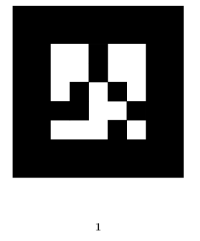
\includegraphics[scale=0.75]{pic/numberedMarker.png}
\caption{Shows an AlvarTag with corresponding ID}
\label{fig:smartAlvarFlow}
\end{figure}

To identify the Alvar Tag, a webcam is used to take a picture of the tag. The picture is evaluated by an algorithm, offered by the Alvar Library, which maps the tag to and specific ID. If the lookup table stored in the component holds the ID of the scanned Alvar Tag, the appropriate marker is returned. Markers hold the information about the color of the owning team, type of station and the side (front or back). 


\subsubsection{Changes in 2018}

Because the component worked well at the RoboCup 2017, only minimal adjustments were made. The version of 2017 returns after one evaluation of the Alvar Tag with a message whether a tag was found or not. The Instruction Planner kept triggering the component up to five times, to ensure that the reason for no tag ID is not the quality of the picture. 
This repetition, done by the Instruction Planner is now moved into the SmartAlvarTagDetection component. Because the task of the component is to offer an ID out of an AlvarTag, it is reasonable to repeat the procedure up to a maximum number of tries (five times) in the component itself.


\subsubsection{Testing}

The component can still be tested in the isolated DeployAlvarTest deployment. Because of the minimal changes in the component, it was not necessary to test the component in an isolated deployment. The new component is integrated in the master deployment for the RoboCup 2018 and has been tested there. It found in most of the cases the correct ID of the AlvarTag on the machine.
The former team has tested the component in the DeployAlvarTest deployment. Their outcome was that the distance of the webcam to an AlvarTag should not be more than six meters. The robot should also facing the AlvarTag in a way, 
%%unverst�ndlich%%%

The angle to the AlvarTag from the webcam should not be more than 45 or 120 degree.